\chapter{Preparazione TAE e Restrizione del DNA}

\vspace{0.6cm}


\section{Sommario}

\subsection{Scopo}

Quest'esperienza in laboratorio si divide in due fasi:

\begin{itemize}

	\item Restrizione del DNA

	\item Preparazione delle componenti per l'elettroforesi

\end{itemize}

Durante la fase di Restrizione del DNA dobbiamo fare in modo che all'interno del
plasmide pUC18 venga inserito il gene di interesse e quello per la resistenza all'ampicillina.
\vspace{0.3cm}

Durante la fase di preparazione dei componenti per l'elettroforesi invece bisognerà preparare il gel di
agarosio, dove poi andranno a correre le due concentrazioni di plasmide, uno digerito e l'altro non digerito.

\subsection{Cenni teorici}

\textbf{Enzimi di restizione}
\vspace{0.3cm}



Gli enzimi di restrizione sono degli enzimi endonucleasici che tagliano le molecole
di DNA a doppio filamento in siti specifici, chiamati siti di restrizione,
che si trovano all'interno o adiacenti a sequenze di nucleotidi chiamate siti di riconoscimento.
Questi enzimi riconoscono anche sequenze di DNA palindromiche, cioè sequenze che lette sia
partendo da 5' che dal 3' sono identiche.

Gli enzimi di restizione producono due diversi tipi di estremità nel DNA:
\begin{itemize}

	\item Estremità piatte, nel caso di enzimi di restrizione che tagliano i filamenti esattamente
	nell'asse di simmetria della sequenza palindromica (Clunt ends);
	\item Estremità protruding(overhangs) a singolo filamento(stickly ends), nel caso degli enzimi di
	restizione che tagliano ogni filamento in posizione similare ai lati opposti dell'asse di simmetria.

\end{itemize}

l'enzima di restizione da noi usato è \textbf{EcoR I}, questo crea 4 estremità
adesive(stickly ends) nucleotide con  5'end  di AATT. La sequenza di riconoscimento
degli acidi nucleici in cui l'enzima taglia è G / ​​AATTC, che ha una sequenza
palindromica complementare di CTTAA / G.

\vspace{0.5cm}


\textbf{Elettroforesi }

\vspace{0.3cm}



L'elettroforesi su gel di agarosio, da noi utilizzata in questa esperienza, è un
metodo semplice e veloce che permette di separare e quindi di identificare
frammenti di DNA in base al loro peso molecolare.

I gel più utilizzati per questa tecnica sono 2:
\begin{itemize}

	\item{Gel di poliacrilamide: } Usualmente usati per separare frammenti di
	DNA inferiori a 500pb ed hanno un elevata risoluzione, ma sono però più complicati
	e pericolosi da preparare e più difficili da maneggiare rispetto a quelli fatti con agarosio.

	\item{Gel di agarosio: } Sono semplici da preparare e sono tipicamente usati per
	separare frammenti di dimensioni variabili, da poche centinaia di basi fino a 20 Kb.
	Essi sono i più diffusi e maggiormente utilizzati per l'analisi di routine su DNA.
	L'agarosio è un polimero di carboidrati estratto dalle alghe.
	Esso, se fuso e gelificato, forma una matrice la cui porosità dipende dalla concentrazione di agarosio.

\end{itemize}

Dopo la loro polimerizzazione, i gel vengono posti nelle apposite vaschette elettroforetiche,
riempite in seguito dal buffer di corsa.
Questo tampone è lo stesso e alla stessa concentrazione di quello usato per polimerizzare l'agarosio.
\vspace{0.3cm}
I tamponi più usati sono:
\begin{itemize}

\item{TAE (Tris-acetato +EDTA): }
Questo nel tempo perde la capacità tamponante perchè si ha la separazione
di cariche agli elettrodi. Viene utilizzato quasi sempre alla concentrazione 1X.

\item{TBE (Tris-borato + EDTA):}
Ha capacità tamponante superiore al TAE.
\`E stabile e usato in corse elettroforetiche particolarmente lunghe,
ma con il tempo tende a precipitare.
Può essere utilizzato ad una concetrazione di 0.5X perchè già a questa
concentrazione ha un potere tamponante sufficiente.

\item{TPE (Tris-fosfato + EDTA).}

 \end{itemize}

Il Tris contenuto nel tampone è un sale che tampona tra pH 7 e pH 8, range dove il DNA
si mantiene molto bene. L'EDTA invece è un chelante che sequestra ioni Mg\textsuperscript{2+}
presenti in soluzione che vengono utilizzati da enzimi che degradano il DNA (DNAsi).

Il principio di funzionamento dell'elettroforesi consiste nel movimento di particelle
cariche negativamente, DNA, RNA o proteine(saturate con SDS cioè Sodio-dodecilsolfato),
in un campo elettrico verso il polo positivo (anodo).

La separazione avviene in base alle dimensioni e quindi alla massa della molecola.
La distanza di migrazione è maggiore per molecole piccole, le quali sono trattenute meno dalla maglia
polissaccaridica formata dal gel.

Un altro aspetto importante per la corsa elettroforetica è il tempo,
che è direttamente proporzionale alla risoluzione. Si può però velocizzare il processo
aumentando il voltaggio, ma bisogna fare attenzione a non incorrere nei rischi del
calore prodotto per l'effetto Joule.

\begin{figure}[H]

	\centering
	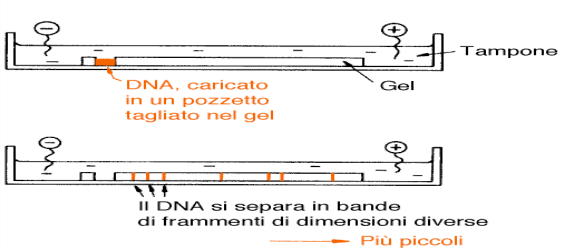
\includegraphics[width=0.6\textwidth]{./immagini/elettroforesi.png}
	\caption{Elettroforesi su GEL}
	\label{elettroforesi}

\end{figure}

\subsection{Materiali utilizzati}

\begin{itemize}
	\item Guanti in lattice
	\item Micropipette (\SI{100}{\micro\liter}-\SI{1000}{\micro\liter} e \SI{2}{\micro\liter}-\SI{200}{\micro\liter})
	\item Beuta da laboratorio
	\item Forno a micronde
	\item Strumenti per l'elettroforesi
	\item Eppendorf
\end{itemize}

\subsection{Soluzioni utilizzate}

\begin{itemize}

	\item Miniprep del pUC18
	\item Enzima di restrizione EcoR I
	\item Acqua
	\item Buffer 10X(digestione)
	\item TAE 50X
	\item SyberSafe
	\item Marker (DNA Ladder)

\end{itemize}

\section{Procedimento}

\subsection{Restrizione del DNA}

\begin{enumerate}

	\item prelevare \SI{10}{\micro\liter} di pUC18 e metterli in una nuova eppendorf
	ed altri \SI{11.5}{\micro\liter} da mettere in un'ulteriore eppendorf per effettuare in
	una provetta la reazione (con l'enzima) e nell'altra il controllo negativo (senza l'enzima).

	\item Addizionare alla eppendorf contenente il nostro plasmide,
	prima \SI{11.5}{\micro\liter} di H\textsubscript{2}O, successivamente
	\SI{2.5}{\micro\liter} di buffer 10X ed infine \SI{1}{\micro\liter} del nostro enzima di restizione EcoR I.

	\item Portare la eppendorf contenente la reazione ad una temperatura di 37°C
	(Temperatura ottimale per l'enzima di restrizione EcoR I) per 1-2 ore,
	in modo che l'enzima EcoR I possa compiere la sua catalizzazione.

\end{enumerate}

\subsection{Preparazione ed Elettroforesi}


\begin{enumerate}

	\item Per prima cosa si procede preparando il gel di agarosio 0.8\%, prendendo una beuta
	ed aggiungendo a questa 0.6 g di agarosio, 1.6 ml di TAE 50X e 78.4 ml di H\textsubscript{2}O
	in modo da avere un volume totale di 80 ml.

	\item La miscela a questo punto si presenterà con l'agarosio in fase solida,
	poichè a temperatura ambiente non è solubile.
	Dobbiamo perciò portare la soluzione ad una temperatura prossima all'ebollizione.
	Andremo quindi a scaldare il tutto all'interno di un forno a micronde, prestando attenzione
	che la soluzone non bolla per più di qualche secondo.

	\item Una volta estratta la beuta, facendo attenzione al calore,
	la si mescola fino a che non si otterrà una soluzione omogenea in contenuto e colore.

	\begin{figure}[H]
		\centering
		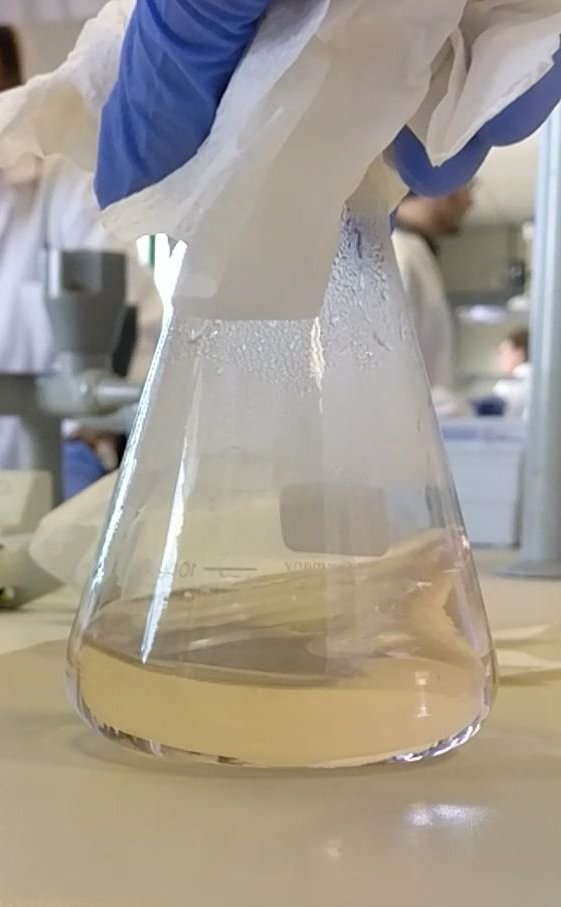
\includegraphics[width=0.3\textwidth]{./immagini/agarosio.jpg}
		\caption{Mescolamento della soluzione con agarosio}
		\label{agarosio}

	\end{figure}

	\item Una volta che la soluzione risulta omogenea e la sua temperatura \`e calata,
	si va ad aggiungere \SI{5}{\micro\liter} di SyberSafe.
	Questo serve come intercalante che si va a legare alla doppia elica
	e sottoposto a raggi UV si rende visibile grazie alla sua fluorescenza.

	\item Andiamo a versare la soluzione nella vaschetta apposita che,
	solidificandosi, ne prende la forma.
	Bisogna inserire il pettine all'interno della vaschetta,
	finch\`e il gel non ha ancora solidificato.
	In questo modo si creeranno i pozzetti dove si andrà a mettere il contenuto delle
	due eppendorf preparate in precedenza una volta che il gel risulter\`a solidificato.

	\begin{figure}[H]

		\centering
		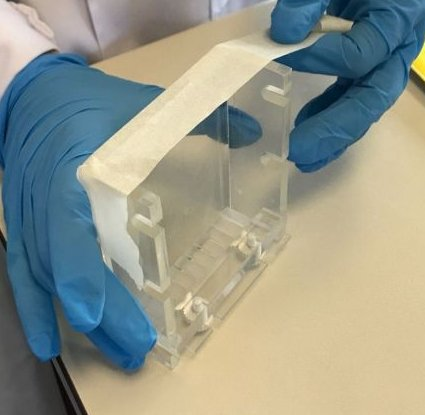
\includegraphics[width=0.3\textwidth]{./immagini/vaschetta.jpg}
		\caption{Vaschetta per solidificazione del gel di agarosio}
		\label{vaschetta}

	\end{figure}


	\item Non appena il gel si sarà solidificato, porlo nella vaschetta togliendo il pettine.
	\item Aggiungere 250 ml di buffer di corsa(TAE 1X) fino al livello indicato.
	\item Caricare all'interno dei pozzetti le varie soluzioni per la corsa elettroforetica tra cui:

	\begin{itemize}

		\item \SI{25}{\micro\liter} di pUC18 digerito (con \SI{5}{\micro\liter} di Loading Buffer)
		\item \SI{25}{\micro\liter} di pUC18 non digerito (con \SI{5}{\micro\liter} di Loading Buffer)
		\item \SI{25}{\micro\liter} di RNA totale derivante dalla scorsa esperienza
		(con \SI{5}{\micro\liter} di Loading Buffer)
		\item Un pozzetto è riservato per il Marker.

	\end{itemize}

	\begin{figure}[H]
		\centering
		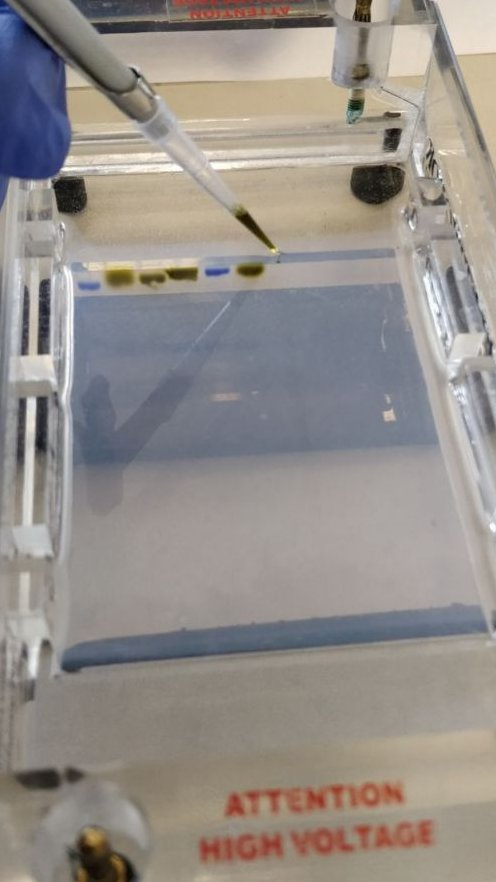
\includegraphics[width=0.3\textwidth]{./immagini/caricamento.jpg}
		\caption{Fase di caricamento dei pozzetti}
		\label{cricamento}
	\end{figure}

	Il Marker è un composto da una miscela di frammenti lineari di DNA con dimensioni
	note che migrano nel gel in prevedibile.
	In questo modo, \`e possibile confrontare il campione con il marker,
	determinando approssimativamente la lunghezza del frammento.

	Il Loading buffer è un colorante con velocità di migrazione nota,
	aggiunto ai composti inseriti nei pozzetti in modo da poter seguire
	l'andamento dell'elettroforesi.

	\begin{figure}[H]

		\centering
		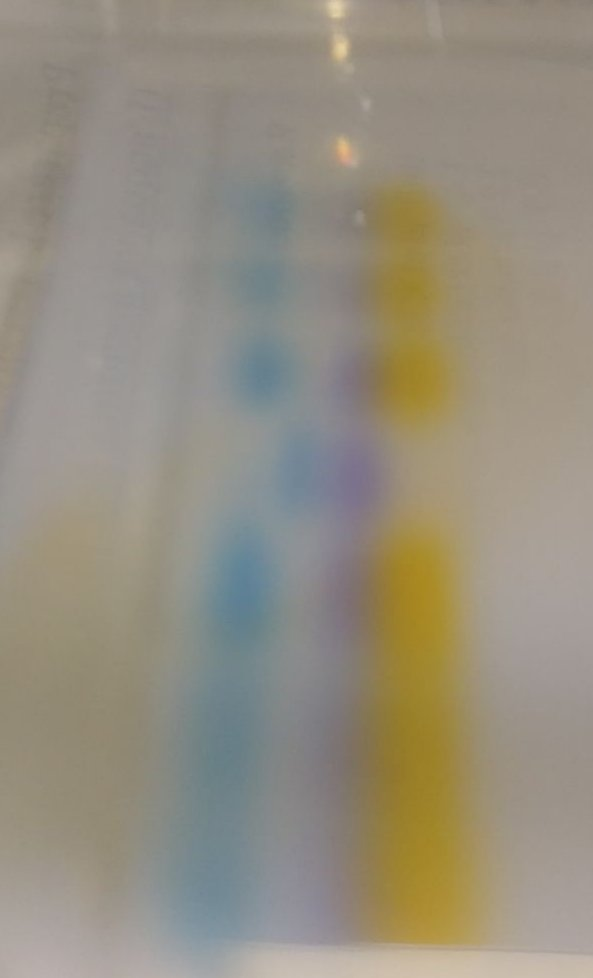
\includegraphics[width=0.3\textwidth]{./immagini/separazione.jpg}
		\caption{Divisione delle bande colorate (Loading buffer)}
		\label{loading_buffer}

	\end{figure}

	\item Caricati i pozzetti chiudere la scatola per l'elettroforesi ed azionare la corrente,
	aspettando il tempo necessario affinch\`e bande risultino ben separate.

	\item Finita la corsa elettroforetica, prendere il gel e metterlo su una piastra
	che emana raggi UV. Coprire con una lastra di vetro che non permetta la fuoriuscita dei raggi UV,
	in modo da non danneggiare gli occhi.
	Avviare la macchina che emette radiazioni UV, in modo da vedere le bande dove il DNA \`e localizzato.
	Confrontandolo con le bande del marker, si pu\`o capire la lunghezza dei vari frammenti.

	\begin{figure}[H]

		\centering
		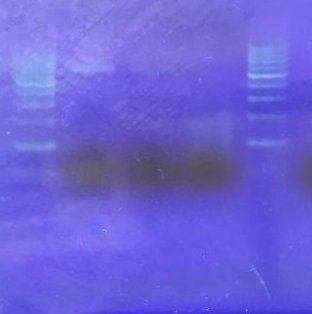
\includegraphics[width=0.3\textwidth]{./immagini/uv.jpg}
		\caption{Fluorescenza del SyberSafe (DNA)}
		\label{SyberSafe}

	\end{figure}



\end{enumerate}


\section{Risultati e Conclusioni}

Durante questa esperienza abbiamo capito il funzionamento dell'elettroforesi nei suoi passaggi,
tra cui la preparazione del gel di agarosio, la preparazione e la colorazione delle soluzioni,
il caricamento nei pozzetti di queste e la successiva fluorescenza data dai raggi UV.

Abbiamo compreso poi il processo di digestione tramite gli enzimi di restrizione,
nel nostro caso l'enzima EcoR I.

Andando a guardare l'immagine risultante dalla fluorescenza,
possiamo notare come nei nostri pozzetti,
la quantità di DNA è molto bassa rispetto al
marker (all'interno del primo pozzetto e del sesto pozzetto).
Questo può essere causato da una poca quantità di materiale, oppure qualche errore nella procedura.
Confrontando con le bande del marker possiamo capire all'incirca le dimensioni dei nostri frammenti.
